% vim: set foldmethod=marker foldlevel=0:

\documentclass[a4paper]{article}
\usepackage[UKenglish]{babel}

\usepackage{preamble}
\usepackage{tikz}

\fancyhead[L]{CS147 Assignment 2}
\title{CS147 Discrete Maths and its Applications 2, Assignment 2}
\colorlet{questionbodycolor}{orange!50}

\begin{document}

\maketitle

\setlength{\parindent}{0em}
\setlength{\parskip}{1em}

% {{{ Q1
\question{1}

\begin{questionbody}
Consider any matching $M \subseteq E$ in a graph $G = (V, E)$. Consider any subset of edges $Z \subseteq M$. Is the following statement true or false? Justify your answer.

The set of edges $Z$ must also form a matching in $G$.
\end{questionbody}

A matching is just a set of edges in $G$ which do not share any common endpoint. For $Z$ to not be a matching, we would need to choose two edges from $M$ which share a node. Since $M$ is a matching, no such pair of edges exists by definition, so $Z$ must also be a matching.

% }}}

% {{{ Q2
\newquestion{2}

\begin{questionbody}
Consider any graph $G = (V, E)$ with $|V| = n$ nodes, where each node $v \in V$ is incident on exactly two edges in $E$. Is the following statement true or false? Justify your answer.

There must exist a matching $M \subseteq E$ in $G$ with $|M| \ge \df n2$.
\end{questionbody}

%By Euler's handshaking lemma, there must be $n$ edges.
The graph is isomorphic to an $n$-gon. For example, the case of $n=4$ could be drawn as a square.

In the case of even $n$, there must exist two maximum matchings of size $\df n2$, which are complements of each other in $E$, so $M_2 = E \setminus M_1$.

In the case of odd $n$, we still get two complementary matchings, but they are not large enough. Take the case of $n=5$ for example,

\begin{center}
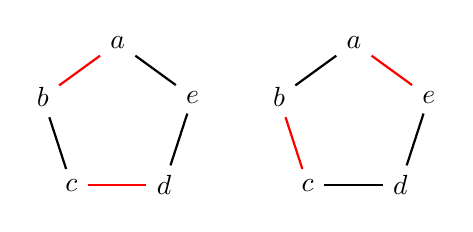
\begin{tikzpicture}[
	every path/.style={thick},
]
	\node (a) at (90:1) {$a$};
	\node (b) at (162:1) {$b$};
	\node (c) at (234:1) {$c$};
	\node (d) at (306:1) {$d$};
	\node (e) at (18:1) {$e$};

	\draw [red] (a) -- (b);
	\draw (b) -- (c);
	\draw [red] (c) -- (d);
	\draw (d) -- (e);
	\draw (e) -- (a);

	\node (a) at ([xshift=3cm]90:1) {$a$};
	\node (b) at ([xshift=3cm]162:1) {$b$};
	\node (c) at ([xshift=3cm]234:1) {$c$};
	\node (d) at ([xshift=3cm]306:1) {$d$};
	\node (e) at ([xshift=3cm]18:1) {$e$};
                        
	\draw (a) -- (b);   
	\draw [red] (b) -- (c);
	\draw (c) -- (d);
	\draw (d) -- (e);
	\draw [red] (e) -- (a);
\end{tikzpicture}
\end{center}

Both of the subsets highlighted in red are matchings, but both are maximum and of size 2. It is clear that in the case of odd n, a maximum matching has size $\l\lfloor \df n2 \r\rfloor$.

Therefore it is false that there must exist a matching $M \subset E$ with $|M| \ge \df n2$.

% }}}

% {{{ Q3
\newquestion{3}

\begin{questionbody}
Let $M \subseteq E$ be a \textit{maximal} matching in a graph $G = (V, E)$, i.e., $M$ is a matching, and furthermore, every edge $(u, v) \in E \setminus M$ has at least one endpoint that is matched under $M$. Let $M^* \subseteq E$ be a matching of \textit{maximum} size in $G$. Is the following statement true or false? Justify your answer.

We must have $|M| \ge \f12 |M^*|$.
\end{questionbody}

Suppose we have a situation where $|M| < \f12 |M^*|$. Let $|M| = \ell$ and $|M^*| = k$ so that $M$ matches $2\ell$ nodes and $M^*$ matches $2k$ nodes. The inequality implies $\ell < \f12 k \iff 2\ell < k$.

There are at most $2\ell$ edges in $M^*$ which are matched by $M$. But since $2\ell < k$, there is at least one edge in $M^*$ which is not matched by $M$. Therefore we can add this edge to $M$, meaning it is not maximal. That's a contradiction, therefore $|M| < \f12 |M^*|$.

% }}}

% {{{ Q4
\newquestion{4}

\begin{questionbody}
Consider a bipartite graph $G = (L \cup R, E)$ where each edge $e \in E$ has one endpoint in $L$ and the other endpoint in $R$. For each set of nodes $X \subseteq L$, let $N_G(X)$ = $\l\{v \in R \colon \text{there is an edge } (u, v) \in E \text{ for some } u \in X \r\}$ denote the set of neighbours of $X$ in $G$.

The graph $G$ has the property that $|N_G(A)| \ge \f12 |A|/2$ for all $A \subseteq L$. Is the following statement true or false? Justify your answer. 

There is a subset of edges $H \subseteq E$ in $G$ which satisfy the three properties described below:
\vspace*{-1em}
\begin{itemize}
	\item[--] $|H| = |L|$.
	\item[--] Every node $u \in L$ is incident upon exactly one edge from $H$.
	\item[--] Every node $v \in R$ is incident upon at most two edges from $H$.
\end{itemize}
\end{questionbody}

To satisfy the first two properties, we require that $H$ is constructed by considering each node in $L$ and choosing one of the edges that connects to it.

Is it possible that there exists a $v \in R$ which is incident on three edges in $H$? Suppose such a $v$ does exist. Then those three edges in $H$ would connect to three distinct nodes in $L$, call them $S = \{u_1, u_2, u_3\}$. But by the neighbour requirement of $G$, we have $|N_G(S)| \ge \f12 |S|$.

By construction, all three nodes connect to the same $v \in R$ and no other nodes, so $N_G(S) = 1$. Therefore we have $1 \ge \f32$, which is a contradiction.

Therefore we cannot have a $v \in R$ which is incident on three edges in $H$. Therefore every node in $R$ is incident on at most two edges in $H$, so the statement is true.

% }}}

\end{document}
